% Part 2 chapter carrying "Dual-Sector Expansion: Type Ia Supernovae ..." (23 Feb 2026), read in full 2026-10-02 (re-confirmed in 50-line chunks, ledger 1-1239, no gaps), in the paper's order.
% Checks and reproduction: docs/verification/chains/DUAL_SECTOR_VALIDATION_CHECK.md, docs/verification/scripts/verify_dual_sector_validation.py.
% Conclusions stated directly: two results (LCDM supernova geometry; beta on supernova distances excluded).

\chapter{Type Ia supernovae in the dual-sector picture: $\Lambda$CDM distances with a locally calibrated $H_0$}\label{ch:dsvalidation}
Two results stand: supernova distances follow $\Lambda$CDM geometry ($\beta_{\rm distance}=-0.035$, $68\,\%$ interval $-0.065$ to $0.000$, full
covariance) \observed, and the $\beta$ term applied to supernova distances is excluded ($\Delta\chi^2=+23.6$) \calc.

\section{The question}
The CMB gives $H_0=67.4\pm0.5$ km\,s$^{-1}$\,Mpc$^{-1}$ (Planck 2018~\cite{Planck2018VI}); the Cepheid-calibrated distance ladder gives $73.04\pm1.04$ (SH0ES, Riess et al.\ 2022~\cite{Riess2022}).
In the dual-sector picture the late-time coupling acts on matter and not on light, with $\beta_m=\Omega_m/2=0.15765$ from the virial partition and no free
parameter beyond $\Lambda$CDM. The Level 2 chains (Chapter~\ref{ch:dual}) give $\Delta\chi^2=+0.54$ against $\Lambda$CDM, $\sigma_8$ from $0.809$ to $0.800$ \fitted, and the
split $H_0^{\rm photon}=67.16$, $H_0^{\rm matter}=67.16\sqrt{1.15765}=72.26$ \calc. Supernovae are hosted in galaxies and calibrated on Cepheids in nearby galaxies;
the question is what the Pantheon+ supernovae themselves say about the two sectors.

\section{Framework}
The matter-sector expansion rate is
\begin{equation}
H_m^2(a)=H_0^2\left[\Omega_ma^{-3}+\Omega_\Lambda+\beta E(a)\right],\qquad E(a)=\exp(1-1/a),
\end{equation}
while the background Friedmann equation, which sets photon paths, is $\Lambda$CDM. Two predictions for supernovae follow:
\begin{enumerate}
\item \emph{Normalisation.} The local calibration reads the matter-sector rate, $72.26$ \prediction. The Cepheid ladder gives $73.04\pm1.04$~\cite{Riess2022}, $0.75\sigma$ above it; the tip of the red giant branch gives $70.39\pm1.94$~\cite{Freedman2025}, $0.97\sigma$ below it \observed.
\item \emph{Geometry.} The shape of $d_L(z)$ follows $\Lambda$CDM ($\beta_{\rm distance}\approx0$), because the coupling acts on growth, not on the background.
\end{enumerate}
Mapped to the $\mu$--$\Sigma$ parameterisation, $\mu(a)=H^2_{\Lambda\rm CDM}/(H^2_{\Lambda\rm CDM}+\beta_mE(a)H_0^2)$ and $\Sigma=1$: $\mu=0.864$ today, $0.982$ at $z=1$,
$\to1$ above $z\approx3$. \calc

\section{Data and method}
Pantheon+SH0ES (Brout et al.\ 2022~\cite{Brout2022,Scolnic2022}): 1701 light curves, $0.001<z<2.26$; the Hubble flow $z>0.01$ leaves 1588 supernovae (1590 with the collaboration's
$z_{\rm HD}$). The model magnitude is $m_b=M+5\log_{10}(d_L/10\,{\rm pc})$, with $d_L=(1+z)\int_0^z c\,dz'/H(z')$ and $M$ free. We first fit
$(\Omega_m,H_0,\beta,M)$ with diagonal errors and three $H_0$ priors: Planck (Test A), SH0ES (Test B), none (Test C), and then use the full
statistical-plus-systematic covariance.

\section{What the three tests show}\label{sec:dsv_tests}
\calc\ $H_0$ and $M$ enter the magnitudes only as $M-5\log_{10}H_0$. With $M$ free the supernova $\chi^2$ is therefore independent of $H_0$: it is $721.12$ at
$H_0=67.4$, $70$ and $73.04$ alike, with $M-5\log_{10}H_0=-28.935$ each time. The $H_0$ in Tests A and B is the prior, absorbed by $M$; Test C's drift to the edge
of the $H_0$ range is the same flat direction. Tests A and B reach the same best fit ($\Omega_m=0.205$, $\beta=-0.30$, $\chi^2=721.12$). The supernova magnitudes alone therefore cannot choose between $67.4$ and $73.04$.
$H_0=73.04$ is set by the Cepheid calibration of $M$, which is the measurement the dual-sector picture assigns to the matter sector.
\begin{figure}[htbp]\centering
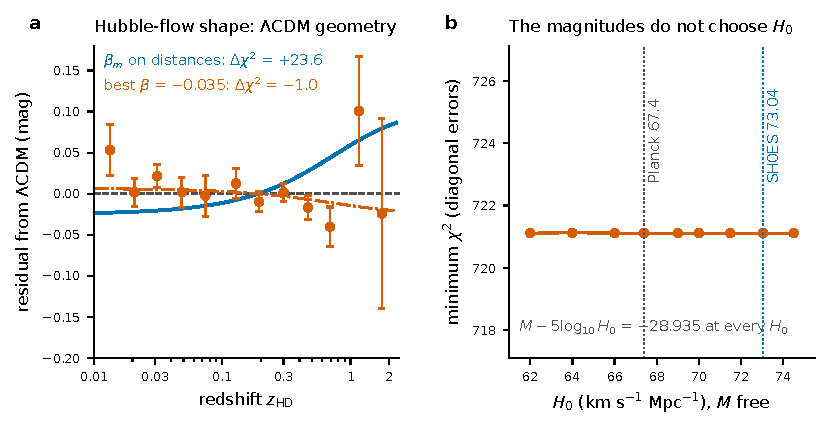
\includegraphics[width=\textwidth]{figures/part2/fig_sn_h0_flat.pdf}
\caption[Pantheon+: the Hubble-flow shape and the flat $H_0$ direction]{Pantheon+SH0ES~\cite{Brout2022,Scolnic2022}. (a) Hubble-flow residuals ($z_{\rm HD}>0.01$, 1590 supernovae) from $\Lambda$CDM at $\Omega_m=0.315$, the offset $M$ fitted with the full statistical and systematic covariance; points are inverse-variance means of the diagonal errors in bins of $\log z$. Solid: $\beta_m=0.15765$ put into the distances ($\Delta\chi^2=+23.6$); dash-dotted: the best $\beta=-0.035$; each curve carries its own fitted offset. (b) Minimum $\chi^2$ at fixed $H_0$ with $M$, $\Omega_m$ and $\beta$ free (diagonal errors, $0.01<z_{\rm CMB}<2.5$, 1588 supernovae): flat at 721.12, with $M-5\log_{10}H_0=-28.935$ at every $H_0$. The magnitudes alone do not choose between 67.4 and 73.04. Method of \texttt{docs/verification/scripts/\allowbreak{}verify\_dual\_sector\_validation.py}. \observed\ \calc}\label{fig:sn_h0_flat}
\end{figure}
With $M$ free, the supernova fits can neither reject the photon-sector expansion rate nor confirm the matter-sector $H_0$; the evidence for
Prediction~1 is the SH0ES calibration itself. \observed

\section{What the supernovae do measure: geometry}

\begin{figure}[htbp]\centering
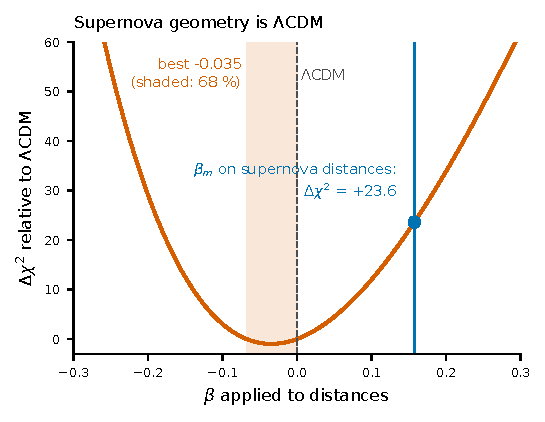
\includegraphics[width=0.62\textwidth]{figures/part2/fig_sn_beta.pdf}
\caption{Pantheon+SH0ES, 1590 Hubble-flow supernovae ($z_{\rm HD}>0.01$), full statistical and systematic covariance, $M$ marginalised, $\Omega_m=0.315$: $\Delta\chi^2$ against $\Lambda$CDM when $\beta E(a)$ is put into the distances. Best $\beta=-0.035$ (68\,\%: $-0.065$ to $0.000$, shaded); the full coupling $\beta_m=0.15765$ on the distances costs $\Delta\chi^2=+23.6$. Method of \texttt{docs/verification/scripts/\allowbreak{}verify\_dual\_sector\_validation.py}. \observed}\label{fig:sn_beta}
\end{figure}
\observed\ With the full covariance and $M$ marginalised, the shape of the Hubble diagram at Planck's $\Omega_m=0.315$ gives $\beta=-0.035$ ($68\,\%$: $-0.065$ to
$0.000$). Supernova distances follow $\Lambda$CDM geometry: Prediction~2 holds. As a sanity check, $\Lambda$CDM with $\Omega_m$ free returns $\Omega_m=0.330$,
matching the Pantheon+ result ($0.334\pm0.018$~\cite{Brout2022}).
\calc\ Applying the full matter-sector rate $H_m(z)$ to supernova distances worsens the fit by $\Delta\chi^2=+23.6$ at $\Omega_m=0.315$ (it can be offset only with
$\Omega_m=0.41$). The data therefore favour the reading in which the supernovae carry the matter-sector \emph{normalisation} through their calibration and
$\Lambda$CDM \emph{geometry} through their Hubble-flow shape, which is the reading of the two predictions above. The Level 1 Planck + Pantheon+ chains,
with the background unmodified, agree: $\Delta\chi^2=+1.58$ (Chapter~\ref{ch:latetime}).

\section{Growth versus geometry}
The coupling's main effect is on growth. The matter density fraction
\begin{equation}
\Omega_m(a;\beta)=\frac{\Omega_ma^{-3}}{\Omega_ma^{-3}+\Omega_\Lambda+\beta E(a)}<\Omega_m(a;0)
\end{equation}
enters the growth equation and lowers $\sigma_8$ ($0.809\to0.800$ in the Level 2 chains); $f\sigma_8(z)$ from SDSS, BOSS and eBOSS~\cite{Howlett2015,Alam2017,Alam2021} probes it directly. Distances
integrate the background $H(z)$, which is unchanged.

\section{Alternatives}
\paragraph{Supernova systematics.} Photometry, dust and calibration systematics move $M$, and through it the ladder $H_0$; the Hubble-flow shape is protected by
the full covariance used above.
\paragraph{Early dark energy.} It raises the CMB-inferred $H_0$ by shrinking the sound horizon, does not split the sectors, and tends to raise $S_8$ (Hill et al.\ 2020~\cite{Hill2020}).
\paragraph{Generic modified gravity.} $f(R)$, normal-branch DGP and most scalar--tensor theories give $\mu>1$ or correlated changes in $\mu$ and $\Sigma$.
The self-accelerating branch of DGP gives $\mu<1$ with $\Sigma=1$, but it carries a ghost~\cite{Koyama2007} and is in tension with CMB,
supernova and $H_0$ data~\cite{Fang2008}. The dual-sector picture gives $\mu<1$ with $\Sigma=1$ and an unmodified background.

\section{Consistency across observables}
\begin{center}\small
\begin{tabularx}{\linewidth}{>{\raggedright\arraybackslash}X>{\raggedright\arraybackslash}X>{\raggedright\arraybackslash}X}\hline
Observable & Sector & Value\\\hline
CMB acoustic scale, Planck $H_0$ & photon & $67.16$ (Level 2 chain); $\beta_\gamma<0.0039$\\
$f\sigma_8$ (SDSS, BOSS, eBOSS) & matter, growth & $\sigma_8\ 0.809\to0.800$\\
BAO angles & photon paths & unchanged (Chapter~\ref{ch:latetime})\\
Cepheid-calibrated ladder (SH0ES) & matter, normalisation & $73.04\pm1.04$; predicted $72.26$\\
Pantheon+ Hubble-flow shape & geometry & $\beta=-0.035^{+0.035}_{-0.030}$, $\Lambda$CDM\\\hline
\end{tabularx}
\end{center}
\calc\ Photon sector. Applying the full coupling $\beta=0.1577$ to photon paths, with the sound horizon and all other parameters fixed, moves the acoustic
scale by $+0.90\,\%$, or $30\sigma$ at Planck's precision~\cite{Planck2018VI} ($\sigma_{\theta_s}=3.1\times10^{-6}$). Fitting a separate photon coupling to $\theta_s$ gives
$\beta_\gamma<0.0039$ (95\,\%), so $\beta_\gamma/\beta_m<0.025$: photons couple at under $2.5\,\%$ of the matter coupling. With every parameter free, the CMB
can absorb a background change only by moving $H_0$ to $\approx61.5$ (Level 2b runs), which BAO and the distance ladder exclude.

\section{Predictions}
\begin{enumerate}
\item \emph{CMB-S4}~\cite{Abazajian2016}: a tighter acoustic-scale constraint on any photon-sector coupling. \prediction
\item \emph{Weak lensing (Euclid, LSST)}~\cite{Euclid2025,Ivezic2019}: $S_8=\sigma_8\sqrt{\Omega_m/0.3}=0.822$ for the Level 2 chain ($\sigma_8=0.800$, $\Omega_m=0.3166$), with $\Sigma=1$. \prediction
\item \emph{DESI Year 5}: the projected aggregate precision on $f\sigma_8$ over all redshifts is $0.74\,\%$ ($k_{\max}=0.1\,h$\,Mpc$^{-1}$) to $0.38\,\%$
($0.2\,h$\,Mpc$^{-1}$)~\cite{DESI2016}, against a predicted deficit of $1.35$--$2.17\,\%$ at $z=0.3$--$0.5$. \prediction
\item \emph{Standard sirens}: binary-neutron-star hosts are galaxies, so sirens read the matter-sector rate, $72.26$. \prediction\ With one event so far,
analyses of GW170817 range from $70.0^{+12.0}_{-8.0}$~\cite{Abbott2017Siren} to $75.5^{+5.3}_{-5.4}$~\cite{Palmese2024}, consistent with both rates. \observed
\item \emph{Euclid} $\mu_0$: the prediction is $\mu_0=-0.136$. Euclid's published forecasts bracket the test of the IAM $\mu(z)$ from about $0.3\sigma$ (conservative scale cuts) to about $7\sigma$ (smallest
scales modelled), and a forecast made with the IAM $\mu(z)$ itself is still to be done (Chapter~\ref{ch:latetime}). \prediction
\end{enumerate}
